% arara: lualatex: { synctex: yes, shell: yes, interaction: nonstopmode }
% arara: biber
% arara: lualatex: { synctex: yes, shell: yes, interaction: nonstopmode }
% arara: lualatex: { synctex: yes, shell: yes, interaction: nonstopmode }
%
%
%                               ,--,              
%          ,---._             ,---.'|              
%       .-- -.' \   ,----..  |   | :   .--.--.    
%       |    |   : /   /   \ :   : |  /  /    '.  
%       :    ;   ||   :     :|   ' : |  :  /`. /  
%       :        |.   |  ;. /;   ; ' ;  |  |--`   
%       |    :   :.   ; /--` '   | |_|  :  ;_     
%       :         ;   | ;    |   | :.'\  \    `.  
%       |    ;   ||   : |    '   :    ;`----.   \ 
%   ___ l         .   | '___ |   |  ./ __ \  \  | 
%  /    /\    J   :'   ; : .'|;   : ;  /  /`--'  / 
% /  ../  `..-    ,'   | '/  :|   ,/  '--'.     /  
% \    \         ; |   :    / '---'     `--'---'   
%  \    \      ,'   \   \ .'                       
%   "---....--'      `---`                         
%                   
%                                 Journal of 
%                                 Computational
%                                 Literary Studies
%                                
%                                 https://jcls.io
%
% Template for authors
%
% Structure of this template:
% .
% ├── README.md
% ├── acknowlegements.tex <-- acknowledgements, funding information
% ├── figures             <-- images and pictures
% ├── fonts               <-- needed fonts 
% ├── jcls.cls            <-- the latex document class
% ├── logos               <-- the journal logos
% ├── main.tex            <-- your content
% ├── metadata            
% │   ├── article.tex     <-- metadata provided by the journal editors
% │   ├── self.bib        <-- metadata provided by the journal editors
% │   └── authors.tex     <-- metadata provided by the authors
% └── references.bib      <-- your biblatex bibliography
%
% This document needs to be compiled with
% LuaLaTeX + Biber
%
%

\documentclass{jcls}
%
%
% The documentclass already loads a number of packages, amongst others:
% - amsmath,amssym
% - xcolor, graphicx
% - babel, csquotes
% - biblatex
% - fontspec, microtype
% - booktabs, longtable
% - listings
%
% -----------------------------------------------

\title{Unnecessarily Complicated Research Title}
\subtitle{A subtitle, if you like}
\shorttitle{Complicated Research}
%
%
% \title and \shorttitle are mandatory, \subtitle can be omitted
%
% 

%
%
% In order to anonymise your submission, the information on authors and 
% affiliations have to be provided in the file: authors.tex
%
% Thanks and acknowledgements and funding
% information have to be saved in: acknowledgements.tex
% These information will also be anonymised automatically 
%

\keywords{computational, literary, studies}
%
%
% 4-6 meaningful keywords that describe the paper



\dataavailability{Data can be found here: \url{data.example.edu/data}}
\softwareavailability{Software can be found here: \url{github.com/something}}
%
%
% Please anonymise your repositories with https://anonymous.4open.science/ or similar services 
%
%


\addbibresource{references.bib}
%
%
% Save all your references in this Bib(La)TeX file
%
%


\begin{document}
\maketitle

\begin{abstract}
	Max. 150 words. Lorem ipsum dolor sit amet, consectetur adipiscing elit. Vestibulum in metus hendrerit, tempus leo nec, convallis metus. Ut gravida, ipsum ac imperdiet condimentum, lacus massa luctus libero, in viverra ante sapien quis velit. Praesent ornare, lectus ac convallis rhoncus, ex elit fermentum urna, vel luctus enim ligula et odio. In nec iaculis libero, vel luctus est. Praesent a massa ut eros rutrum condimentum. Nulla varius, ligula sed tempor fermentum, lorem metus sollicitudin tellus, eget laoreet justo nulla non dolor. Maecenas tempor in est quis eleifend. Vivamus mollis tempor arcu vel convallis. Cras rhoncus, metus id aliquam gravida, quam elit iaculis quam, et porta nisi magna a nibh. Nam tincidunt non urna quis rutrum. Integer a felis blandit, posuere diam a, laoreet risus.
\end{abstract}

\section{Introduction}

Maecenas quis mauris et quam porta faucibus sit amet vel ex. Suspendisse eget facilisis urna, ac accumsan nisl. Curabitur semper posuere convallis. Etiam vitae felis eget nisi maximus rhoncus. Aenean sagittis egestas nisi, a ultrices mauris fringilla vel. Donec accumsan, metus vel lobortis feugiat, dolor erat tempus elit, quis pretium lacus erat ut odio. Integer mattis suscipit tincidunt.\footnote{This is a footnote}

This document is an example, two items are cited: \textit{The \LaTeX\ Companion} book: \cite[see][12-14]{latexcompanion}. And Einstein's journal paper: \cite{einstein}.

Vivamus vestibulum lacinia laoreet. Pellentesque eu porta massa, a posuere odio. Praesent dolor risus, porta ac ornare ut, lacinia quis est. Orci varius natoque penatibus et magnis dis parturient montes, nascetur ridiculus mus. Etiam molestie auctor rutrum. Maecenas nec ornare metus. Nullam varius convallis enim, ut egestas erat condimentum eget. Phasellus lacinia ligula eget nisl feugiat mollis. Donec a ornare felis. Nulla ex dui, semper vitae diam sit amet, ornare viverra justo. Interdum et malesuada fames ac ante ipsum primis in faucibus. In placerat, tellus non consequat blandit, est enim accumsan lacus, ac auctor purus sapien nec lorem. Aliquam bibendum dolor ut volutpat rhoncus .

\section{Meaningful title}

Donec viverra bibendum ante vel faucibus. Maecenas vitae laoreet libero, vitae posuere dolor. Phasellus luctus, neque in pharetra faucibus, tellus sapien mollis libero, sed elementum turpis ex nec justo. Ut molestie enim nec ipsum scelerisque maximus. Sed tincidunt risus commodo neque hendrerit, eu scelerisque nisl dignissim. Praesent et varius velit. Donec dictum sed sem vel fermentum. Suspendisse convallis nunc varius, volutpat sem quis, gravida metus.

\begin{figure}
	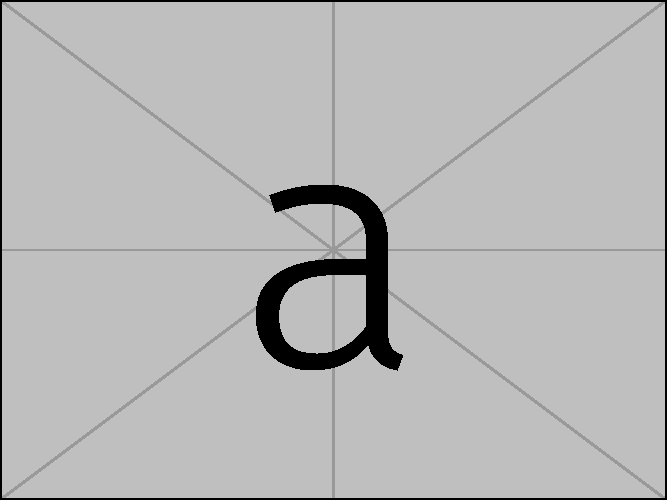
\includegraphics[width=\linewidth]{image-a.pdf}
	\caption{Image a}
\end{figure}
%
%
% Images should be put in the directory: figures
%
%

\subsection{Subsection}

Class aptent taciti sociosqu ad litora torquent per conubia nostra, per inceptos himenaeos. Morbi egestas vestibulum tortor. Mauris tempus nec nisl ut lacinia. Quisque congue nunc non ornare dapibus. Proin sit amet porttitor erat, eget varius mauris. Donec feugiat ligula ac enim cursus molestie. Donec tempor in lectus at facilisis. Vivamus pulvinar finibus lectus fringilla sodales. Nam fringilla ut velit quis commodo. Ut in velit sed dui euismod fringilla. Aliquam condimentum commodo purus ac suscipit. Donec auctor turpis libero, eu ultricies nisl hendrerit et. Nam gravida hendrerit tortor sit amet sagittis (\cite{dirac}).

\subsubsection{Math}

The well known Pythagorean theorem $x^2 + y^2 = z^2$ was proved to be
invalid for other exponents. Something else is
\(\forall x \in X, \quad \exists y \leq ε\).

And display math:
\[
	\int_a^b x^2  \mathrm{d} x
\]

\subsubsection{Code}

This is some very trivial python code:

\begin{lstlisting}[language=Python]
def backwards(string):
    return string[::-1]

def is_palindrome(string):
    if string == backwards(string): 
		return True

A <- www >>= B  # This is a comment
\end{lstlisting}

\section{Tables}

\begin{table}[ht]
	\begin{tabular}{@{}lllll@{}}
		Value & Something & Other & T & F \\ \midrule
		1     & 2         & 3     & a & b \\
		4     & 5         & 6     & c & d \\
		7     & 8         & 9     & e & f \\
	\end{tabular}
	\caption{A table}
\end{table}

If your table is too big to fit on one page, you can also use the longtable environment:

\begin{fullwidth}
	\begin{longtable}{@{}llllll@{}}
		written     & burn        & orange   & share      & quick       & slowly    \\* \midrule
		\endhead
		%
		\endfoot
		%
		\endlastfoot
		%
		stronger    & slightly    & fat      & new        & enemy       & represent \\
		development & deal        & putting  & supper     & greatly     & thy       \\
		nice        & suddenly    & origin   & age        & almost      & tone      \\
		managed     & highest     & function & pig        & include     & fly       \\
		phrae       & could       & just     & giant      & over        & horn      \\
		separate    & obtain      & mail     & apart      & pole        & origin    \\
		toy         & please      & vast     & cowboy     & bean        & birthday  \\
		say         & region      & couple   & how        & screen      & dust      \\
		nest        & surface     & fence    & at         & related     & child     \\
		stared      & horn        & farmer   & mighty     & raise       & vessels   \\
		did         & forgot      & twice    & number     & advice      & also      \\
		daughter    & suit        & far      & image      & arrangement & funny     \\
		bad         & bar         & poem     & themselves & safe        & skin      \\
		curve       & comfortable & identity & composed   & attack      & some      \\
		long        & signal      & certain  & bring      & seems       & baby      \\
		system      & leaving     & myself   & aware      & himself     & except    \\
		smell       & combination & courage  & victory    & telephone   & white     \\
		interior    & balance     & helpful  & former     & drove       & general   \\
		freedom     & noun        & wall     & outline    & other       & park      \\
		nice        & suddenly    & origin   & age        & almost      & tone      \\
		managed     & highest     & function & pig        & include     & fly       \\
		phrase      & could       & just     & giant      & over        & horn      \\
		separate    & obtain      & mail     & apart      & pole        & origin    \\
		toy         & please      & vast     & cowboy     & bean        & birthday  \\
		say         & region      & couple   & how        & screen      & dust      \\
		nest        & surface     & fence    & at         & related     & child     \\
		stared      & horn        & farmer   & mighty     & raise       & vessels   \\
		development & deal        & putting  & supper     & greatly     & thy       \\
		nice        & suddenly    & origin   & age        & almost      & tone      \\
		managed     & highest     & function & pig        & include     & fly       \\
		did         & forgot      & twice    & number     & advice      & also      \\
		daughter    & suit        & far      & image      & arrangement & funny     \\
		bad         & bar         & poem     & themselves & safe        & skin      \\
		curve       & comfortable & identity & composed   & attack      & some      \\
		long        & signal      & certain  & bring      & seems       & baby      \\
		system      & leaving     & myself   & aware      & himself     & except    \\
		smell       & combination & courage  & victory    & telephone   & white     \\
		development & deal        & putting  & supper     & greatly     & thy       \\
		nice        & suddenly    & origin   & age        & almost      & tone      \\
		managed     & highest     & function & pig        & include     & fly       \\
		kitchen     & tin         & motion   & song       & buffalo     & tune      \\
		\caption{A very large table}
	\end{longtable}
\end{fullwidth}

\section{Conclusion}

This is what we found.

%
%
% Acknowledgements, contributions & roles, and references 
% will be set automatically at the end of the document
% Please note: All information in acknowledgement.tex and authors.tex 
% will be anonymized automatically for reviewing
%
\end{document}
